% Created 2017-09-19 Tue 13:43
% Intended LaTeX compiler: pdflatex
\documentclass[11pt]{article}
\usepackage[utf8]{inputenc}
\usepackage[T1]{fontenc}
\usepackage{graphicx}
\usepackage{grffile}
\usepackage{longtable}
\usepackage{wrapfig}
\usepackage{rotating}
\usepackage[normalem]{ulem}
\usepackage{amsmath}
\usepackage{textcomp}
\usepackage{amssymb}
\usepackage{capt-of}
\usepackage{hyperref}
\author{Francesco Antonello Ferraro}
\date{\today}
\title{T1 Autômatos}
\hypersetup{
 pdfauthor={Francesco Antonello Ferraro},
 pdftitle={T1 Autômatos},
 pdfkeywords={},
 pdfsubject={},
 pdfcreator={Emacs 25.1.2 (Org mode 9.0.10)}, 
 pdflang={English}}
\begin{document}

\maketitle
\begin{abstract}
This article aims to show the specificities of the imperative paradigm. As well as making a history background of the reason why the paradigm is wwidely used at classic programming languages, making them behave like they do.
\end{abstract}

\section{Questão 1}
\label{sec:org5d74b37}

\subsection{Letra a}
\label{sec:org77837e9}
\begin{figure}[htbp]
\centering
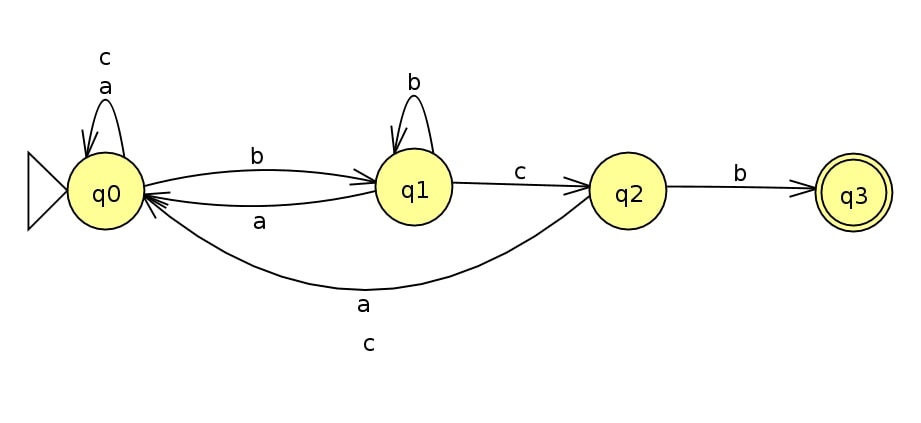
\includegraphics[width=.9\linewidth]{./q1/a/q1a.jpg}
\caption{\label{fig:orgb9c3e39}
Esse é um autômato determinístico}
\end{figure}

\begin{center}
\begin{tabular}{ll}
Input & Result\\
\hline
abcb & Accept\\
bcbb & Reject\\
cbcb & Accept\\
bcbaaa & Reject\\
aaaaa & Reject\\
\end{tabular}
\end{center}

\subsection{Letra b}
\label{sec:org9d5d6e6}
\begin{figure}[htbp]
\centering
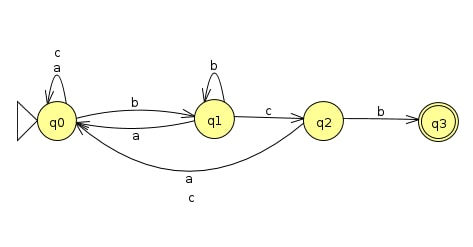
\includegraphics[width=.9\linewidth]{./q1/b/q1b.jpg}
\caption{\label{fig:orgca05c4d}
Esse é um autômato determinístico}
\end{figure}

\begin{center}
\begin{tabular}{ll}
Input & Result\\
\hline
b & Reject\\
a & Reject\\
c & Reject\\
bb & Reject\\
aba & Reject\\
ac & Reject\\
ab & Reject\\
bc & Reject\\
ba & Reject\\
\end{tabular}
\end{center}
\subsection{Letra c}
\label{sec:org973273f}
\begin{figure}[htbp]
\centering
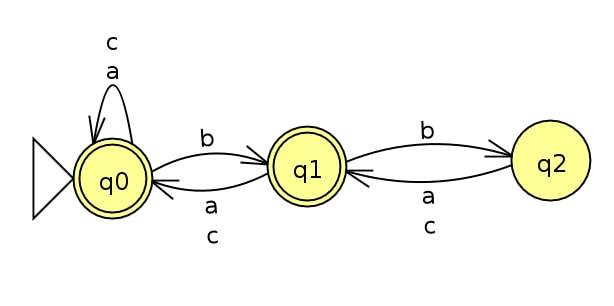
\includegraphics[width=.9\linewidth]{./q1/c/q1c.jpg}
\caption{\label{fig:orgbab1973}
Esse é um autômato determinístico}
\end{figure}

\begin{center}
\begin{tabular}{ll}
Input & Result\\
\hline
aa & Accept\\
bb & Reject\\
cc & Accept\\
c & Accept\\
a & Accept\\
b & Accept\\
aacbacbcba & Accept\\
abcabcbb & Reject\\
\end{tabular}
\end{center}
\subsection{Letra d}
\label{sec:org6837329}
\begin{figure}[htbp]
\centering
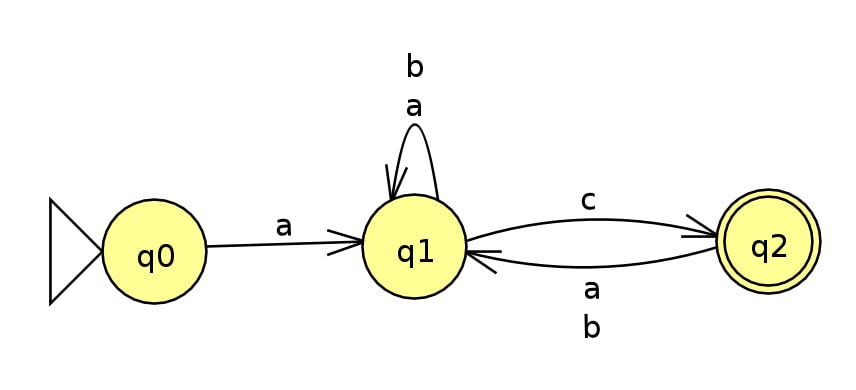
\includegraphics[width=.9\linewidth]{./q1/d/q1d.jpg}
\caption{\label{fig:org492a17c}
Esse é um autômato determinístico}
\end{figure}

\begin{center}
\begin{tabular}{ll}
Input & Result\\
\hline
a & Reject\\
b & Reject\\
c & Reject\\
ac & Accept\\
abcbc & Accept\\
acac & Accept\\
abcbb & Reject\\
\end{tabular}
\end{center}
\end{document}
